% Student Number: 2240357068
% Student Name: Baturay Kafkas
% EEE @ Hacettepe University

% My resource collection: https://github.com/kfksbtry/uni
% Circuits were set up in LTspice.

\documentclass[11pt]{article}

\usepackage{graphicx}
\usepackage[top=25mm, bottom=25mm, left=25mm, right=25mm, a4paper]{geometry}
\usepackage{amsmath}
\usepackage{amssymb}
\usepackage{enumitem}
\usepackage{float}
\usepackage{fancyhdr}
\usepackage{booktabs}
\usepackage{tikz}
\usepackage{steinmetz}
\usepackage{mathrsfs}
\usepackage{cancel}

\pagestyle{fancy}
\fancyhf{}
\fancyhead[R]{Baturay Kafkas - 2240357068 - Electrical \& Electronics Engineering}

\rfoot{\thepage}
\renewcommand{\headrulewidth}{0pt} 
\renewcommand{\footrulewidth}{0pt}
\sloppy

\begin{document}

\begin{center}
\large
\textbf{ELE226 Circuit Theory II Homework 2-3}
\end{center}

\section{Questions}

\

\textbf{Homework 2}

\begin{enumerate}[leftmargin=*,label=\textbf{2.\arabic*.}]

\item \textit{J. W. Nilsson and S. Riedel, Electric Circuits, 10th ed., Pearson, 2014, Assessment Problem 12.2, p. 440}

\item \textit{J. W. Nilsson and S. Riedel, Electric Circuits, 10th ed., Pearson, 2014, Problem 12.13, p. 460}

\item \textit{J. W. Nilsson and S. Riedel, Electric Circuits, 10th ed., Pearson, 2014, Problem 12.20, p. 460}

\item \textit{J. W. Nilsson and S. Riedel, Electric Circuits, 10th ed., Pearson, 2014, Problem 12.22, p. 460}

\item \textit{J. W. Nilsson and S. Riedel, Electric Circuits, 10th ed., Pearson, 2014, Problem 12.24, p. 461}

\item \textit{J. W. Nilsson and S. Riedel, Electric Circuits, 10th ed., Pearson, 2014, Problem 12.40, p. 462}

\item \textit{J. W. Nilsson and S. Riedel, Electric Circuits, 10th ed., Pearson, 2014, Assessment Problem 12.5, p. 447}

\item \textit{J. W. Nilsson and S. Riedel, Electric Circuits, 10th ed., Pearson, 2014, Problem 12.41, p. 462}

\item \textit{J. W. Nilsson and S. Riedel, Electric Circuits, 10th ed., Pearson, 2014, Problem 12.43, p. 463}

\item \textit{J. W. Nilsson and S. Riedel, Electric Circuits, 10th ed., Pearson, 2014, Problem 12.43, p. 463}

\end{enumerate}

\textbf{Homework 3}

\begin{enumerate}[leftmargin=*,label=\textbf{3.\arabic*.}]

\item \textit{J. W. Nilsson and S. Riedel, Electric Circuits, 10th ed., Pearson, 2014, Problem 12.27, p. 461}

\item \textit{J. W. Nilsson and S. Riedel, Electric Circuits, 10th ed., Pearson, 2014, Problem 12.28, p. 461}

\item \textit{J. W. Nilsson and S. Riedel, Electric Circuits, 10th ed., Pearson, 2014, Problem 12.28, p. 461}

\newpage

\item The switch has been in position $a$ for a long time. At $t=0$, it moves to position $b$. Find $i_{L}(t)$ for $t\ge0$. Verify $i_{{L}_{ss}}$ using the phasor approach.

\begin{figure}[H]
    \centering
    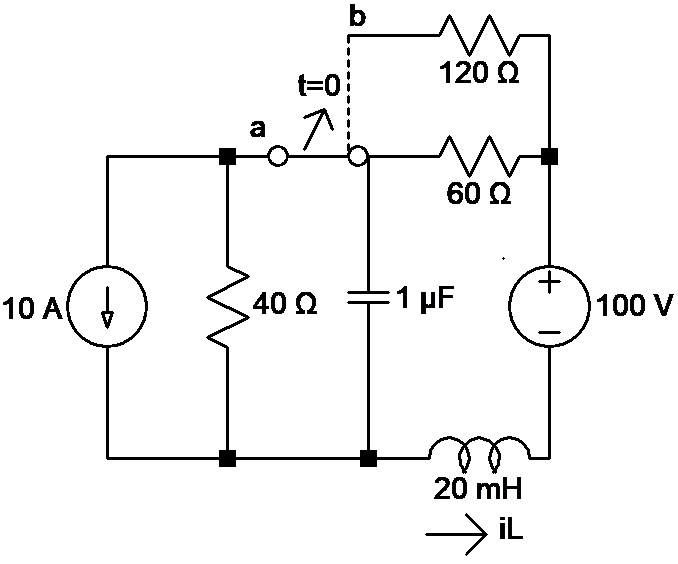
\includegraphics[width=0.45\linewidth]{Q4-1.png}
\end{figure}

\item The capacitor is initially uncharged. Find $I(s)$.

\begin{figure}[H]
    \centering
    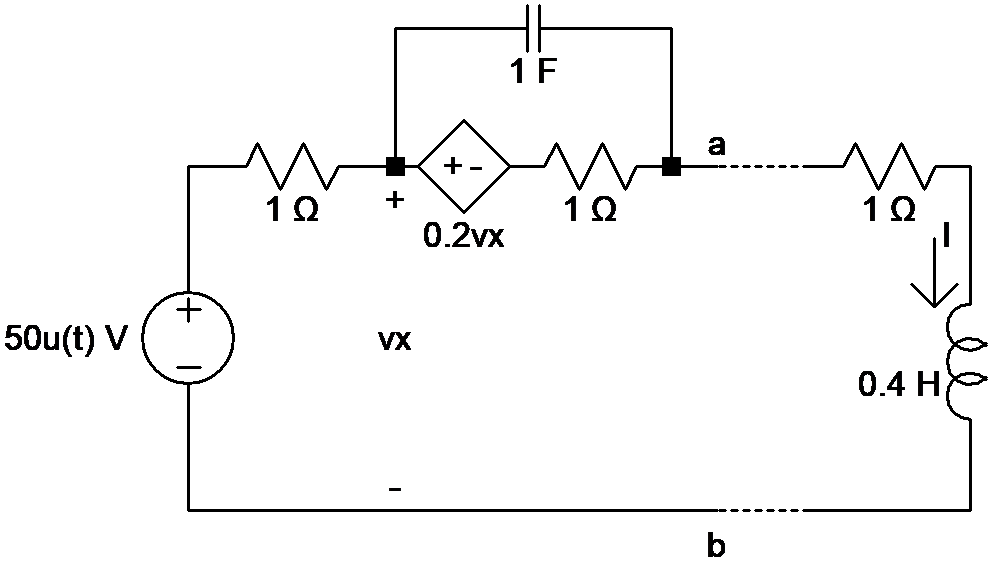
\includegraphics[width=0.55\linewidth]{Q5-1.png}
\end{figure}

\item Find $v(t)$, $t>0$ using the superposition principle.

\begin{figure}[H]
    \centering
    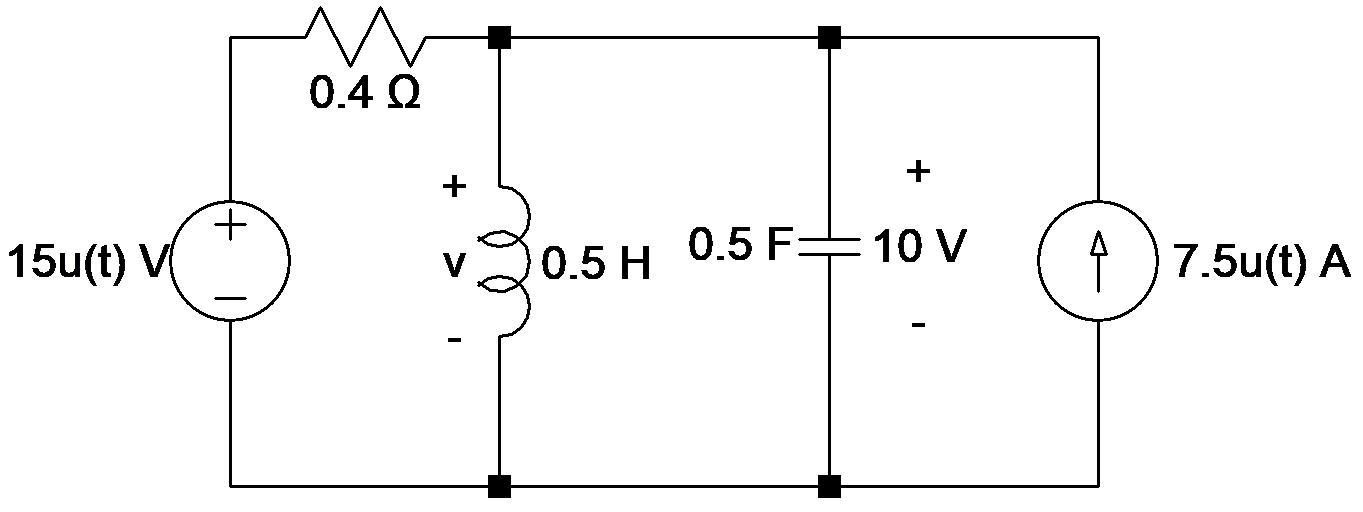
\includegraphics[width=0.6\linewidth]{Q6-1.png}
\end{figure}

\item \textit{J. W. Nilsson and S. Riedel, Electric Circuits, 10th ed., Pearson, 2014, Problem 13.9, p. 505}

\item \textit{J. W. Nilsson and S. Riedel, Electric Circuits, 10th ed., Pearson, 2014, Problem 13.11, p. 505}

\item \textit{J. W. Nilsson and S. Riedel, Electric Circuits, 10th ed., Pearson, 2014, Problem 13.13, p. 506}

\newpage

\item \textit{J. W. Nilsson and S. Riedel, Electric Circuits, 10th ed., Pearson, 2014, Problem 13.14, p. 506}

\item \textit{J. W. Nilsson and S. Riedel, Electric Circuits, 10th ed., Pearson, 2014, Problem 13.17, p. 506}

\item \textit{J. W. Nilsson and S. Riedel, Electric Circuits, 10th ed., Pearson, 2014, Problem 13.20, p. 507}

\item \textit{J. W. Nilsson and S. Riedel, Electric Circuits, 10th ed., Pearson, 2014, Problem 13.23, p. 507}

\item \textit{J. W. Nilsson and S. Riedel, Electric Circuits, 10th ed., Pearson, 2014, Problem 13.28, p. 508}

\item \textit{J. W. Nilsson and S. Riedel, Electric Circuits, 10th ed., Pearson, 2014, Problem 13.29, p. 508}

\item \textit{J. W. Nilsson and S. Riedel, Electric Circuits, 10th ed., Pearson, 2014, Problem 13.30, p. 508}

\item \textit{J. W. Nilsson and S. Riedel, Electric Circuits, 10th ed., Pearson, 2014, Problem 13.32, p. 509}

\item \textit{J. W. Nilsson and S. Riedel, Electric Circuits, 10th ed., Pearson, 2014, Problem 13.35, p. 509}

\item \textit{J. W. Nilsson and S. Riedel, Electric Circuits, 10th ed., Pearson, 2014, Problem 13.36, p. 509}

\item \textit{J. W. Nilsson and S. Riedel, Electric Circuits, 10th ed., Pearson, 2014, Problem 13.36, p. 509}

\end{enumerate}

\newpage

\section{Answers}

\

\textbf{Homework 2}

\begin{enumerate}[leftmargin=*,label=\textbf{2.\arabic*.}]

\item \begin{enumerate}[label=\textbf{\alph*)}]

\item $\mathscr{L}\left\{t^2\right\}=\dfrac{2}{s^3}\implies\mathscr{L}\left\{t^2e^{-at}\right\}=\boxed{\dfrac2{(s+a)^3}}.$
\item $\begin{array}{rl}\mathscr{L}\left\{\dfrac{d}{dt}(e^{-at}\sinh\beta t)\right\}&=s\mathscr{L}\left\{e^{-at}\sinh\beta t\right\}-e^{-at}\sinh\beta t|_{t=0}\\&=s\cdot\dfrac{\beta}{(s+a)^2-\beta^2}-1\cdot0=\boxed{\frac{s\beta}{(s+a)^2-\beta^2}}.\end{array}$
\item $\mathscr{L}\left\{t\cos\omega t\right\}=-\dfrac{d}{ds}\left(\dfrac{s}{s^2+\omega^2}\right)=-\dfrac{s^2+\omega^2-s\cdot2s}{(s^2+\omega^2)^2}=\boxed{\dfrac{s^2-\omega^2}{(s^2+\omega^2)^2}}.$

\end{enumerate}

\item \begin{enumerate}[label=\textbf{\alph*)}]
\item Remember: $\mathscr{L}\left\{g(t-a)u(t-a)\right\}=e^{-as}F(s)$. Let $g(t)=20e^{-500t}$. Then
\[\mathscr{L}\{g(t)\}=\frac{20}{s+500}\implies\mathscr{L}\{g(t-a)u(t-a)\}=\boxed{\frac{20e^{-10s}}{s+500}}\]
\item Rearrange the equation:
\[f(t)=u(t+4)(5t+20)+u(t+2)(-10t-20)+u(t-2)(10t-20)+u(t-4)(5t-20)\]
\[\mathscr{L}\left\{f(t)\right\}=\boxed{5e^{4s}\cdot\frac1{s^2}-10e^{2s}\cdot\frac1{s^2}+10e^{-2s}\cdot\frac1{s^2}+5e^{-4s}\cdot\frac1{s^2}}\]
\end{enumerate}

\item \begin{enumerate}[label=\textbf{\alph*)}]
\item $\mathscr{L}\left\{t\right\}=\dfrac{1}{s^2}\implies\mathscr{L}\left\{te^{-at}\right\}=\boxed{\dfrac1{(s+a)^2}}.$
\item $\mathscr{L}\{f(t)\}=\boxed{\dfrac{w}{s^2+\omega^2}}$
\item Use the formula $\sin(a+b)=\sin a\cos b+\cos a\sin b$.
\[\sin(\omega t+\theta)=\sin(\omega t)\cos\theta+\cos(\omega t)\sin\theta\implies\mathscr{L}\{f(t)\}=\boxed{\dfrac{\omega\cos\theta+s\sin\theta}{s^2+w^2}}\]
\item $\mathscr{L}\{f(t)\}=\boxed{\dfrac{1}{s^2}}$
\item Use the formula $\cosh(a+b)=\cosh a\cosh b+\sinh a\sinh b$.
\[\cosh(t+\theta)=\cosh t\cosh\theta+\sinh t\sinh\theta\implies\mathscr{L}\{f(t)\}=\boxed{\dfrac{s\cosh\theta-\sinh\theta}{s^2-1}}\]
\end{enumerate}

\item \begin{enumerate}[label=\textbf{\alph*)}]
\item $\mathscr{L}\left\{\dfrac{d}{dt}(\sin\omega t)\right\}=s\mathscr{L}\left\{\sin\omega t\right\}-\sin\omega t|_{t=0}=s\cdot\dfrac{\omega}{s^2+\omega^2}-0=\boxed{\frac{s\omega}{s^2+\omega^2}}$.
\item $\mathscr{L}\left\{\dfrac{d}{dt}(\cos\omega t)\right\}=s\mathscr{L}\left\{\cos\omega t\right\}-\cos\omega t|_{t=0}=s\cdot\dfrac{s}{s^2+\omega^2}-1=\boxed{\frac{-\omega^2}{s^2+\omega^2}}.$
\item $\begin{array}{rl}\mathscr{L}\left\{\dfrac{d^3}{dt^3}(t^2u(t))\right\}&=s^3\mathscr{L}\left\{t^2u(t)\right\}-s^2t^2u(t)|_{t=0}-s(t^2u(t))'|_{t=0}-(t^2u(t))''|_{t=0}\\&=s^3\cdot\dfrac{2}{s^3}-0-s(2tu(t)+t^2\delta(t))|_{t=0}-(2u(t)+2t\delta(t))|_{t=0}\\&=\boxed{2}.\end{array}$

\item (a) $\rightarrow\mathscr{L}\{\omega\cos\omega t\}=\omega\mathscr{L}\{\cos\omega t\}=\boxed{\dfrac{s\omega}{s^2+\omega^2}}$.

(b) $\rightarrow\mathscr{L}\{-\omega\sin\omega t\}=-\omega\mathscr{L}\{\sin\omega t\}=\boxed{\dfrac{-\omega^2}{s^2+\omega^2}}$.

(c) $\rightarrow\mathscr{L}\{2\delta(t)\}=2e^{-0s}=\boxed2$.
\end{enumerate}

\item \begin{enumerate}[label=\textbf{\alph*)}]

\item $\begin{array}{rl}\mathscr{L}\left\{\dfrac{d}{dt}(e^{-at}\cos\omega t)\right\}&=s\mathscr{L}\left\{e^{-at}\cos\omega t\right\}-e^{-at}\cos\omega t|_{t=0}\\&=s\cdot\dfrac{s+a}{(s+a)^2+\omega^2}-1=\boxed{\frac{-as-a^2-\omega^2}{(s+a)^2+\omega^2}}.\end{array}$.

\item $\displaystyle\mathscr{L}\left\{\int_{0^-}^te^{-ax}\sin\omega x\,dx)\right\}=\dfrac{\mathscr{L}\{e^{-ax}\sin\omega x\}}{s}=\boxed{\dfrac{w}{[(s+a)^2+\omega^2]s}}$.

\end{enumerate}

\item \begin{enumerate}[label=\textbf{\alph*)}]

\item $F(s)=\dfrac{K_1}{s+5}+\dfrac{K_2}{s+8}$.
\[K_1=\left.\dfrac{6(s+10)}{s+8}\right|_{s=-5}=10,\: K_2=\left.\dfrac{6(s+10)}{s+5}\right|_{s=-8}=-4\:\implies \boxed{f(t)=10e^{-5t}-4e^{-8t}}\]

\item $F(s)=\dfrac{K_1}{s}+\dfrac{K_2}{s+3}$+$\dfrac{K_2}{s+7}$.
\[K_1=\left.\dfrac{20s^2+141s+315}{s^2+10s+21}\right|_{s=0}=15,\: K_2=\left.\dfrac{20s^2+141s+315}{s(s+3)}\right|_{s=-7}=11\]
\[K_3=\left.\dfrac{20s^2+141s+315}{s(s+7)}\right|_{s=-3}=6\implies\boxed{f(t)=15-6e^{-3t}+11e^{-7t}}\]

\item $F(s)=\dfrac{K_1}{s+2}+\dfrac{K_2}{s+4}+\dfrac{K_3}{s+6}$.
\[K_1=\left.\dfrac{15s^2+112s+228}{(s+4)(s+6)}\right|_{s=-2}=8,\:K_2=\left.\dfrac{15s^2+112s+228}{(s+2)(s+6)}\right|_{s=-4}=-5,\]
\[K_3=\left.\dfrac{15s^2+112s+228}{(s+2)(s+4)}\right|_{s=-6}=12\implies \boxed{f(t)=8e^{-2t}-5e^{-4t}+12e^{-6t}}\]

\item $F(s)=\dfrac{K_1}{s}+\dfrac{K_2}{s+1}+\dfrac{K_3}{s+2}+\dfrac{K_4}{s+3}.$
\[K_1=\left.\frac{2s^3+33s^2+93s+54}{(s+1)(s+2)(s+3)}\right|_{s=0}=9,\:K_2=\left.\frac{2s^3+33s^2+93s+54}{s(s+2)(s+3)}\right|_{s=0}=4\]
\[K_3=\left.\frac{2s^3+33s^2+93s+54}{s(s+1)(s+3)}\right|_{s=0}=-8,\:K_4=\left.\frac{2s^3+33s^2+93s+54}{s(s+1)(s+2)}\right|_{s=0}=-3\]
\[\implies\boxed{f(t)=9+4e^{-t}-8e^{-2t}-3e^{-3t}}\]

\end{enumerate}

\item We have $F(s)=\dfrac{K_1}{s+5}+\dfrac{K_2}{s+5-j12}+\dfrac{K_2^*}{s+5+j12}$.

\[K_1=\left.\dfrac{10(s^2+119)}{s^2+10s+169}\right|_{s=-5}=10,\:K_2=\left.\dfrac{10(s^2+119)}{(s+5)(s+5+j12)}\right|_{s=-5+j12}=j4.16\]
\[\implies \boxed{f(t)=10e^{-5t}+8.33e^{-5t}\cos(12t+90^\circ)}\]


\item \begin{enumerate}[label=\textbf{\alph*)}]

\item $F(s)=\dfrac{K}{s+7-j14}+\dfrac{K^*}{s+7+j14}$.
\[K=\left.\dfrac{280}{s+7-j14}\right|_{s=-7-j14}=j10\implies \boxed{f(t)=20e^{-7t}\cos(14t-90^\circ)}\]

\item $F(s)=\dfrac{K_1}{s}+\dfrac{K_2}{s+5-j8}+\dfrac{K_2^*}{s+5+j8}$
\[K_1=\left.\dfrac{-s^2+52s+445}{s^2+10s+89}\right|_{s=0}=5,\:K_2=\left.\dfrac{-s^2+52s+445}{s(s+5+j8)}\right|_{s=-5+j8}=-3+j2\]
\[\boxed{f(t)=5+7.21e^{-5t}\cos(8t-146.31^\circ)}\]

\item $F(s)=\dfrac{K_1}{s+6}+\dfrac{K_2}{s+2-4j}+\dfrac{K_2^*}{s+2+4j}$.
\[K_1=\left.\frac{14s^2+56s+152}{s^2+4s+20}\right|_{s=-6}=10,\:K_2=\left.\frac{14s^2+56s+152}{(s+2+j4)(s+6)}\right|_{s=-2+j4}=2+j2\]
\[\implies\boxed{f(t)=10e^{-6t}+5.66e^{-2t}\cos(4t+45^\circ)}\]

\item $F(s)=\dfrac{K_1}{s+5-j3}+\dfrac{K_1^*}{s+5+j3}+\dfrac{K_2}{s+4-j2}+\dfrac{K_2^*}{s+4+j2}$
\[K_1=\left.\frac{8(s+1)^2}{(s+5+j3)(s^2+8s+20)}\right|_{s=-5+j3}=3.54-j2.97\]
\[K_2=\left.\frac{8(s+1)^2}{(s^2+10s+34)(s+4+2j)}\right|_{s=-4+j2}=-3.54+j0.69\]
\[\boxed{f(t)=9.25e^{-5t}\cos(3t-40.04^\circ)+7.22e^{-4t}\cos(2t+168.93^\circ)}\]
\end{enumerate}.

\item \begin{enumerate}[label=\textbf{\alph*)}]

\item $F(s)=\dfrac{K_1}{s^2}+\dfrac{K_2}s+\dfrac{K_3}{s+8}$.
\[K_1=\left.\dfrac{320}{s+8}\right|_{s=0}=40,\:K_2=\left.\dfrac d{ds}\left(\dfrac{320}{s+8}\right)\right|_{s=0}=-5,\:K_3=\left.\dfrac{320}{s^2}\right|_{s=-8}=5\]
\[\boxed{f(t)=40t-5+5e^{-8t}}\]

\item $F(s)=\dfrac{K_1}{s}+\dfrac{K_2}{(s+2)^2}+\dfrac{K_3}{s+2}$.
\[K_1=\left.\dfrac{80(s+3)}{(s+2)^2}\right|_{s=0}=60,\:K_2=\left.\dfrac{80(s+3)}{s}\right|_{s=-2}=-40\]
\[K_3=\frac d{ds}\left[\dfrac{80(s+3)}{s}\right]_{s=-2}=-60\implies \boxed{f(t)=60-40te^{-2t}-60e^{-2t}}\]

\item $F(s)=\dfrac{K_1}{(s+1)^2}+\dfrac{K_2}{s+1}+\dfrac{K_3}{s+3-j4}+\dfrac{K_4}{s+3+j4}$.
\[K_1=\left.\dfrac{60(s+5)}{s^2+6s+25}\right|_{s=-1}=12,\:K_2=\frac d{ds}\left[\dfrac{60(s+5)}{s^2+6s+25}\right]_{s=-1}=0.6\]
\[K_3=\frac d{ds}\left[\dfrac{60(s+5)}{(s+1)^2(s+3+j4)}\right]_{s=-3+j4}=-0.3+j1.65\]
\[\implies \boxed{f(t)=12te^{-t}+0.6e^{-t}+3.35e^{-3t}\cos(4t+100.305^\circ)}\]

\item $F(s)=\dfrac{K_1}{(s+5)^2}+\dfrac{K_2}{s+5}+\dfrac{K_3}{s^2}+\dfrac{K_4}{s}$.
\[K_1=\left.\dfrac{25(s+4)^2}{s^2}\right|_{s=-5}=1,\:K_2=\frac d{ds}\left[\dfrac{25(s+4)^2}{s^2}\right]_{s=-5}=-1.6\]
\[K_3=\left.\dfrac{25(s+4)^2}{(s+5)^2}\right|_{s=-5}=16,\:K_4=\frac d{ds}\left[\dfrac{25(s+4)^2}{(s+5)^2}\right]_{s=-5}=1.6\]
\[\implies \boxed{f(t)=1.6+16t+te^{-5t}-1.6e^{-5t}}\]

\end{enumerate}.


\item \begin{enumerate}[label=\textbf{\alph*)}]

\item $F(s)=\dfrac{K_1}s+\dfrac{K_2}{(s+3)^3}+\dfrac{K_3}{(s+3)^2}+\dfrac{K_4}{s+3}$.
\[K_1=\left.\dfrac{135}{(s+3)^3}\right|_{s=0}=5,\:K_2=\left.\dfrac{135}{s}\right|_{s=-3}=-45\]
\[K_3=\left.\frac d{ds}\left(\dfrac{135}{s}\right)\right|_{s=-3}=-15,\:2K_4=\left.\frac{d^2}{ds^2}\left(\dfrac{135}{s}\right)\right|_{s=-3}=-10.\implies K_4=-5\]
\[\boxed{f(t)=5-5e^{-3t}-15te^{-3t}-22.5t^2e^{-3t}}\]
\item $F(s)=\dfrac{As+B}{(s^2+2s+2)^2}+\dfrac{Cs+D}{s^2+2s+2}$.
\[10(s+2)^2|_{s=-1+j}=-j20=A(-j+1)+B\implies A=20,\: B=20\]
\[\left.\frac{d}{ds}[10(s+2)]^2\right|_{s=-1+j}=j20+20=A+C(s^2+2s+2)+(Cs+D)(2s+2)|_{s=-1+j}\]
\[\implies C=0,\: D=10.\]
\[\boxed{f(t)=10(t+1)e^{-t}\sin t}\]

\item $F(s)=25+\dfrac{20s+114}{s^2+15s+54}=25+\dfrac{K_1}{s+9}+\dfrac{K_1}{s+6}$
\[K_1=\left.\dfrac{20s+144}{s+6}\right|_{s=-9}=12,\:K_2=\left.\dfrac{20s+144}{s+9}\right|_{s=-6}=8\]
\[\implies\boxed{f(t)=25\delta(t)+8e^{-6t}+12e^{-9t}}\]

\item $F(s)=5s-15+\dfrac{K_1}{s+2}+\dfrac{K_2}{s+5}$
\[K_1=\left.\dfrac{6s+42}{s+5}\right|_{s=-2}=10,\:K_2=\left.\dfrac{6s+42}{s+2}\right|_{s=-5}=-4\]
\[\implies\boxed{f(t)=5\delta'(t)-15\delta(t)+10e^{-2t}-4e^{-5t}}\]

\end{enumerate}

\end{enumerate}

\textbf{Homework 3}

\begin{enumerate}[leftmargin=*,label=\textbf{3.\arabic*.}]

\item \begin{enumerate}[leftmargin=*,label=\textbf{\alph*.}]
\item $\displaystyle\boxed{-I_\text{dc}+\frac1L\int_0^tv_o(\tau)\,d\tau+\frac{v_o}R+C\dfrac{dv_o}{dt}=0}$
\item $\displaystyle\frac{-I_\text{dc}}s+\frac1L\cdot\frac{V_o}s+\frac{V_o}R+CsV_o+\cancel{CV_o( 0)}=0\implies\boxed{V_o(s)=\frac{I_\text{dc}/C}{s^2+\frac s{RC}+\frac1{LC}}\text{ V--s}}$
\item $\displaystyle i_o=C\frac{dv_o}{dt}\implies\boxed{I_o(s)=sCV_o(s)=\frac{sI_\text{dc}}{s^2+\frac s{RC}+\frac1{LC}} \text{ A--s}}$
\end{enumerate}

\item \begin{enumerate}[leftmargin=*,label=\textbf{\alph*.}]
\item $\displaystyle\boxed{\frac{v_o}R+C\frac{dv_o}{dt}+\frac1L\int_0^tv_o(\tau)\,d\tau=0}$
\item We have $\displaystyle\frac LR\frac{di_o}{dt}+LC\frac{d^2i_o}{dt^2}+i_o=0$.
\[\frac LRsI_o-\frac LRI_\text{dc}+LC(s^2I_o-sI_\text{dc}-0)+I_o=0\implies I_o\left(\frac{sL}R+LCs^2+1\right)-I_\text{dc}\left(\frac LR +sLC\right)\]
$\implies\boxed{I_o(s)=\frac{I_\text{dc}\left(s+\frac1{RC}\right)}{s^2+\frac s{RC}+\frac1{LC}}\text{ A--s}}$
\end{enumerate}

\item \begin{enumerate}[leftmargin=*,label=\textbf{\alph*.}]
\item Let $i_o$ circulate in the clockwise direction.
\[Ri_o+L\dfrac{di_o}{dt}+v_o=0\overset{\displaystyle\left[i_o=C\frac{dv_o}{dt}\right]}{\implies}\boxed{\dfrac{d^2v_o}{dt^2}+\dfrac RL\dfrac{dv_o}{dt}+\dfrac{1}{LC}v_o=0}\]
\item From KVL,

\[s^2V_o-sV_\text{dc}-\cancel{v'_o(0)}+\dfrac{R}{L}(sV_o-V_\text{dc})+\dfrac1{LC}V_o=0\implies\boxed{V_o(s)=\dfrac{V_\text{dc}\left(s+\frac RL\right)}{s^2+\frac RLs+\frac1{LC}}\text{ V--s}}\]

\end{enumerate}

\item Initial conditions:
\[i_L(0^-)=5\text{ A},\quad v_C(0^-)=-200\text{ V}.\]

\begin{figure}[H]
    \centering
    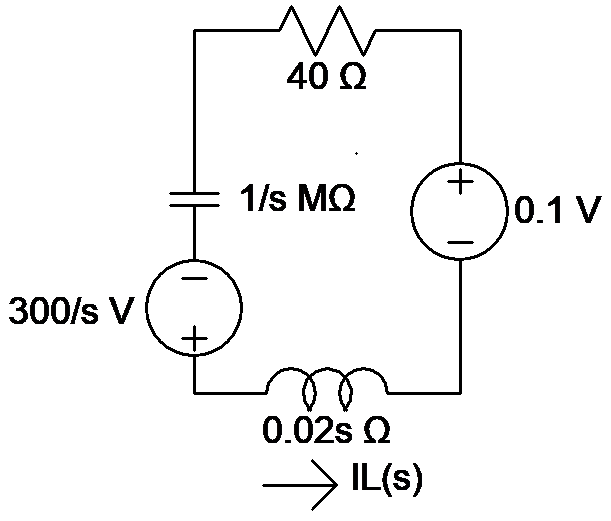
\includegraphics[width=0.4\linewidth]{A4-1.png}
\end{figure}

From KVL,
\[-0.1-\frac{300}s-40I_L+\frac{10^6}{s}I_L+20sI_L\cdot10^{-3}=0\implies I_L=\frac{0.1+\dfrac{300}s}{\dfrac{10^6}s+40+0.02s}\]
\[I_L=\dfrac{5s+15000}{s^2+2000s+50\cdot10^6}=\frac{K_1}{s+1000-j7000}+\frac{K_1^*}{s+1000+j7000}\]
\[K_1=\left.\frac{5s+15000}{s+1000+j7000}\right|_{s=-1000+j7000}z=2.5-j0.714\]
\[\implies\boxed{i_L(t)=[5.2e^{-1000t}\cos(7000t-15.945^\circ)]u(t)\text{ A}}\]

The steady part is $0$ because the capacitor is open at infinity $\left(\omega=0\implies \frac1{j\omega C}\to\infty\right)$, leading to $i_{L_{ss}}=0$.

\item Calculate $\text{V}_{Th}$.
\[\frac{V_x-\dfrac{50}s}{1}+\frac{V_x-V_{Th}}{1/s}+\frac{V_x-0.2V_x-V_{Th}}{1}=0\quad\text{and}\quad V_x=\frac{50}s\]
\[\implies V_{th}=\frac{50s+40}{s+s^2}\]

\begin{figure}[H]
    \centering
    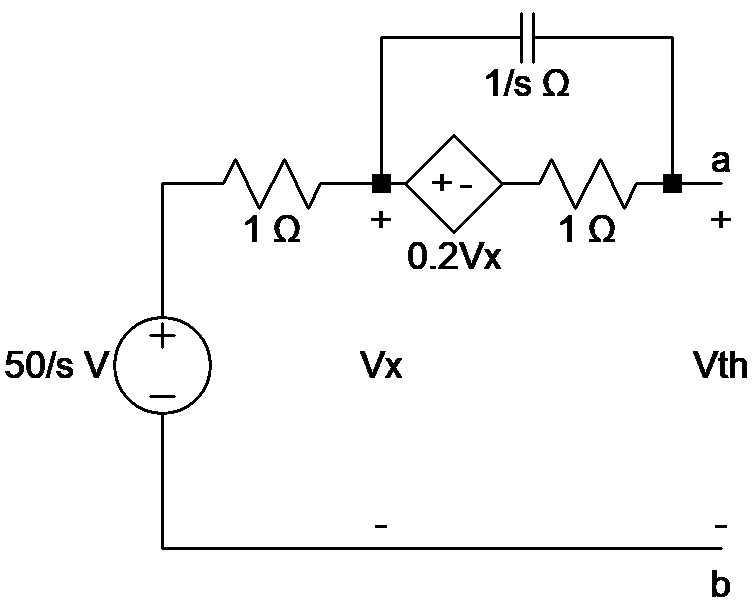
\includegraphics[width=0.5\linewidth]{A5-2.png}
\end{figure}

Zero the $50\text{ V}$ source and apply a test voltage.

\begin{figure}[H]
    \centering
    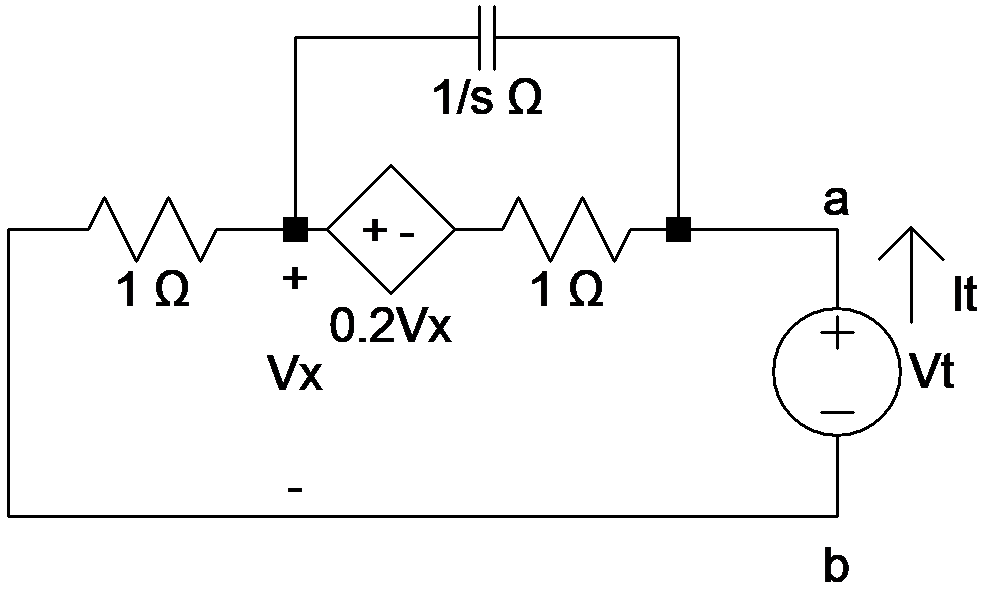
\includegraphics[width=0.5\linewidth]{A5-1.png}
\end{figure}

\[\frac{V_x}1+\frac{V_x-0.2V_x-V_t}1+\frac{V_x-V_t}{1/s}=0\quad\text{and}\quad V_x=i_t\]
\[I_t(2-0.2+s)=V_t(s+1)\implies\frac{V_t}{I_t}=R_{Th}=\frac{1.8+s}{s+1}\]

\[\boxed{I(s)=\frac{\dfrac{50s+40}{s(s+1)}}{1+0.4s+\dfrac{s+1.8}{s+1}}=\frac{125s+100}{s(s^2+6s+7)}\text{ A--s}}\]

\item The $s$--domain equivalent circuit:

\begin{figure}[H]
    \centering
    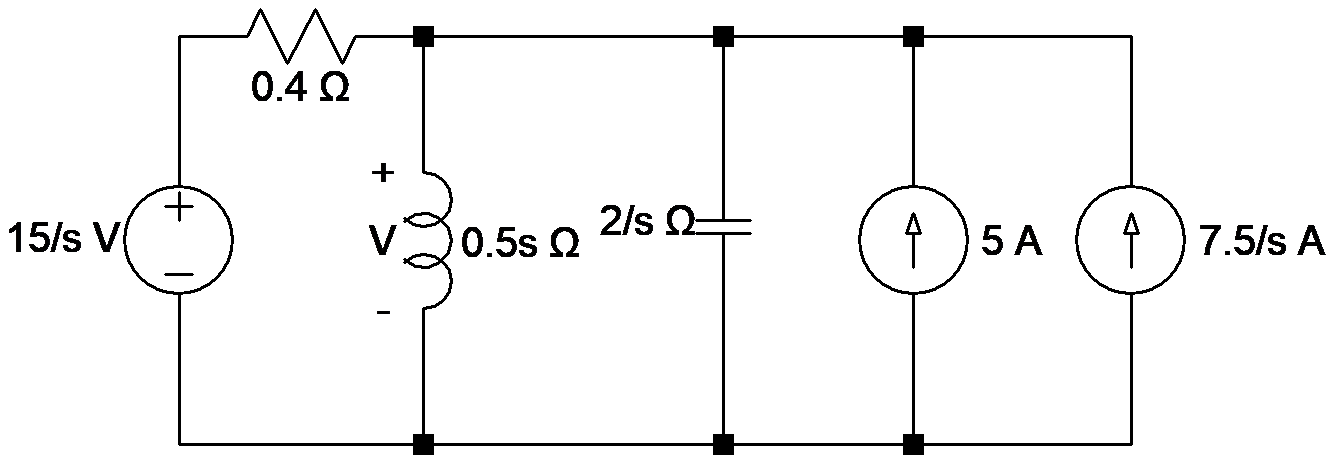
\includegraphics[width=0.65\linewidth]{A6-1.png}
\end{figure}

Zero the current source.

\begin{figure}[H]
    \centering
    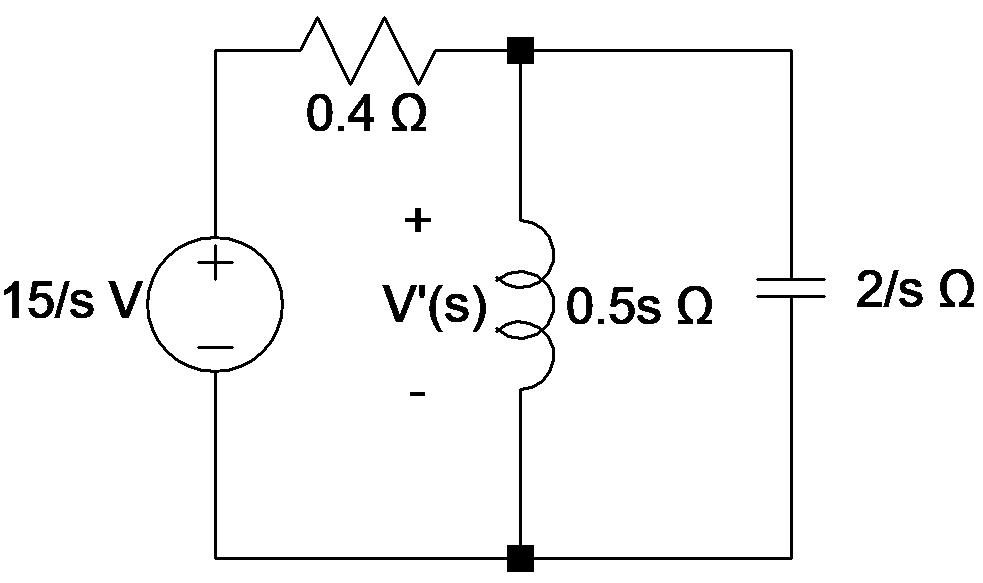
\includegraphics[width=0.55\linewidth]{A6-2.png}
\end{figure}

\[V'(s)=\frac{15}{s}\cdot\frac{0.5s\:\|\:\dfrac2s}{\left(0.5s\:\|\:\dfrac2s\right)+0.4}=\frac{75}{(s+1)(s+4)}=\frac{K_1}{s+1}+\frac{K_2}{s+4}\]
\[K_1=\left.\frac{75}{s+4}\right|_{s=-1}=25,\quad K_2=\left.\frac{75}{s+1}\right|_{s=-4}=-25\implies V'(s)=\frac{25}{s+1}-\frac{25}{s+4}\]

Zero the voltage source.

\begin{figure}[H]
    \centering
    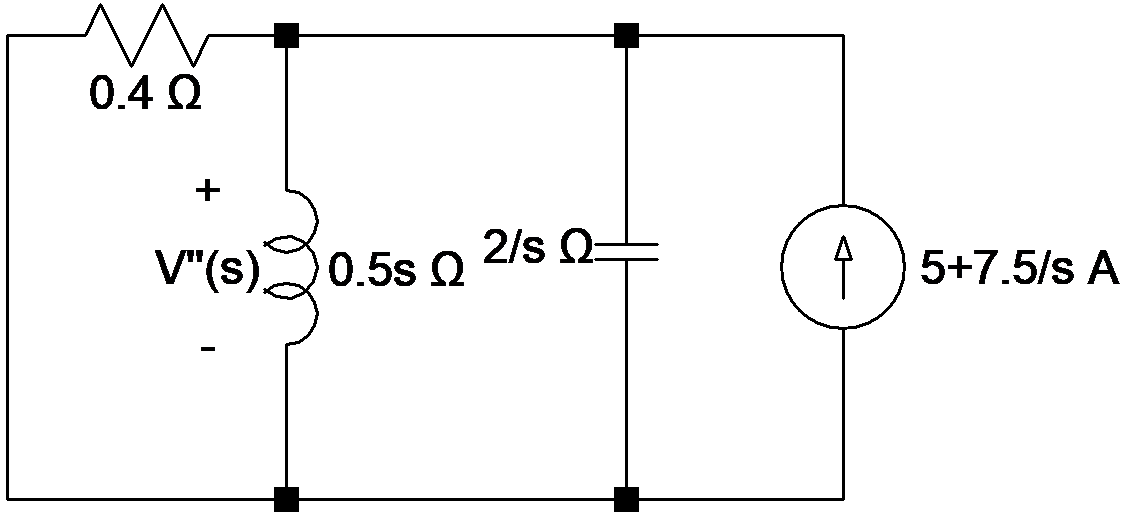
\includegraphics[width=0.6\linewidth]{A6-3.png}
\end{figure}

\[V''(s)=\left(\frac{7.5}{s}\:\|\:s\right)\:\|\:\left(\frac2s\:\|\:0.5s\:\|\:0.4\right)=\frac{2s}{s^2+5s+4}=\frac{K_1}{s+4}+\frac{K_2}{s+1}\]
\[K_1=\left.\frac{15+10s}{s+1}\right|_{s=-4}=\frac{25}3,\quad K_2=\left.\frac{15s+10}{s+4}\right|_{s=-1}=\frac53\implies V''(s)=\frac{25}{3(s+4)}+\frac{5}{3(s+1)}\]

\[V(s)=V'(s)+V''(s)=-\frac{50}3\frac{1}{s+4}+\frac{80}3\frac1{s+1}\implies\boxed{v(t)=\left(-\frac{50}3e^{-4t}+\frac{80}3e^{-t}\right)u(t)\text{ V}}\]

\item Find the $s$--domain circuit.

\begin{figure}[H]
    \centering
    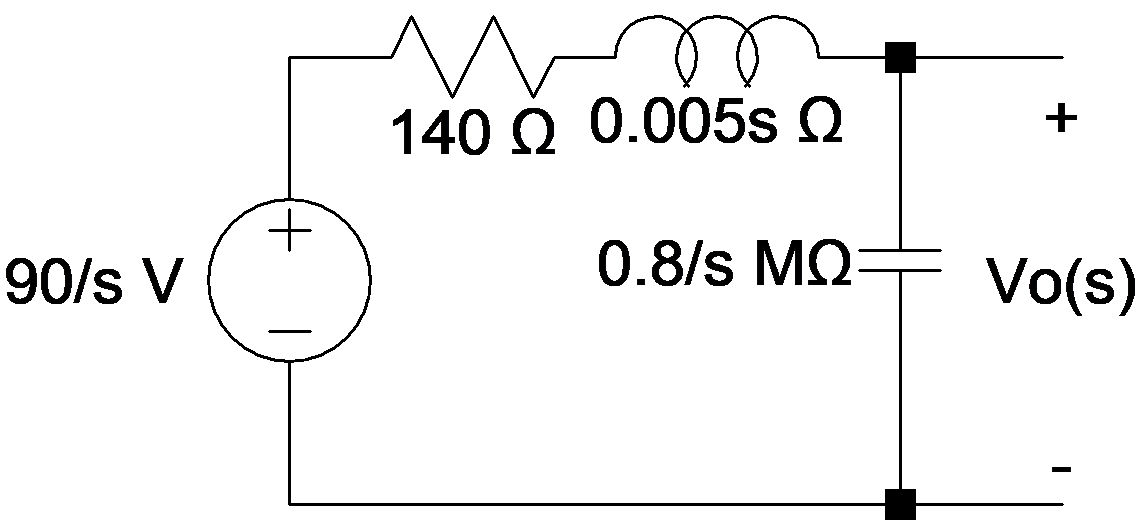
\includegraphics[width=0.5\linewidth]{A7-1.png}
\end{figure}

\[\begin{array}{rl}V_o(s)&=\dfrac{90}s\cdot\dfrac{800000/s}{\dfrac{800000}s+0.005s+140}=\dfrac{90}s\cdot\dfrac{16\cdot10^7}{s^2+28000s+16\cdot10^7}\\&=\dfrac{144\cdot10^8}{s(s+20000)(s+8000)}=\dfrac{K_1}{s}+\dfrac{K_2}{s+20000}+\dfrac{K_3}{s+8000}\end{array}\]
\[K_1=\left.\dfrac{144\cdot10^9}{(s+2000)(s+8000)}\right|_{s=0}=90,\:K_2=\left.\dfrac{144\cdot10^9}{s(s+8000)}\right|_{s=-20000}=60\]
\[K_3=\left.\dfrac{144\cdot10^9}{s(s+20000)}\right|_{s=-8000}=-150\]
\[\implies\boxed{v_o(t)=[90-150e^{-8000t}+60e^{-20000t}] u(t)\text{ V}}\]

\item \begin{enumerate}[label=\textbf{\alph*)}]

\item The circuit:

\begin{figure}[H]
    \centering
    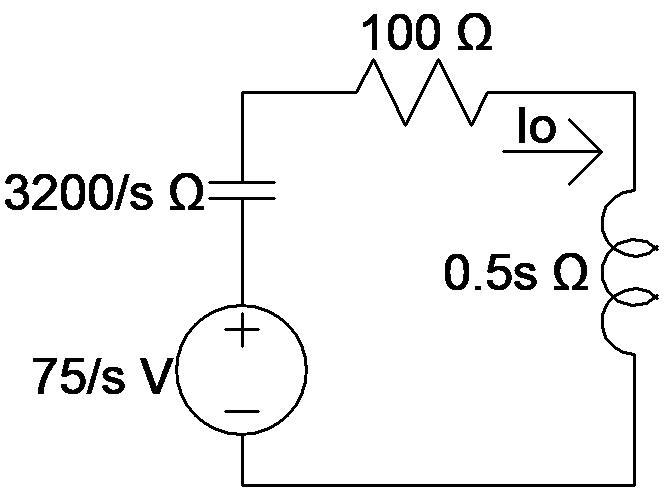
\includegraphics[width=0.35\linewidth]{A8-1.png}
\end{figure}

\item $-\dfrac{75}s+I_o\dfrac{3200}{s}+100I_0+0.5sI_o=0\implies\boxed{I_o(s)=\dfrac{150}{(s+40)(s+160)}\text{ A--s}}$

\item $I_o(s)=\dfrac{K_1}{s+40}+\dfrac{K_2}{s+160}$
\[K_1=\left.\dfrac{150}{s+160}\right|_{s=40}=\frac54,\quad K_2=\left.\dfrac{150}{s+40}\right|_{s=-160}=-\frac54\]
\[\implies\boxed{i_o(t)=\frac54\left(e^{-40t}-e^{-160t}\right)u(t)\text{ A}}\]

\end{enumerate}

\item Find the current through the inductor.

\[-1.25+\frac{v_C}{80}+\frac{v_C}{200}+\frac{v_C-275}{100}=0\implies v_C=150\text{ V},\qquad i_L=\frac{275-150}{100}=1.25\text{ A}\]

\begin{enumerate}[label=\textbf{\alph*)}]

\item The circuit:

\begin{figure}[H]
    \centering
    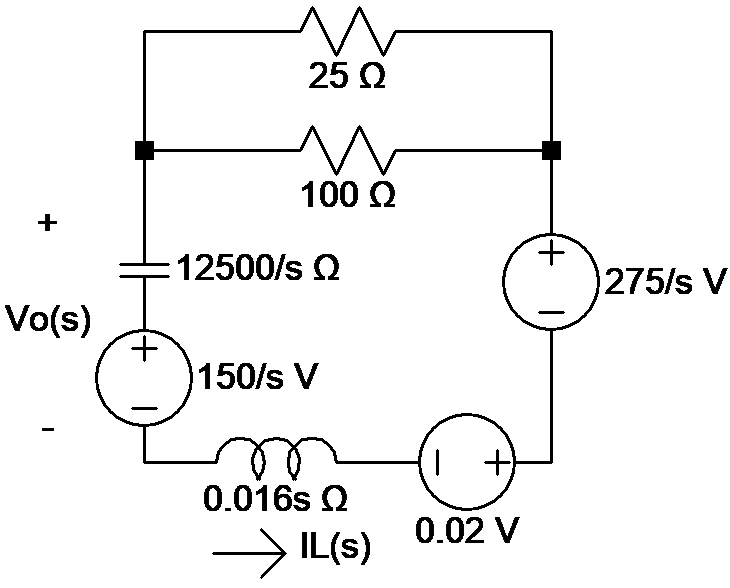
\includegraphics[width=0.4\linewidth]{A9-1.png}
\end{figure}

\item From KCL,
\[0.016sI_L-0.02-\frac{2.75}s+20I_L+\frac{12500}sI_L+\frac{150}s=0\implies I_L=\frac{7812.5+1.25s}{s^2+1250s+781250}\]
\[\boxed{V_o=\frac{12500}sI+\frac{150}s=\frac{150s^2+203125s+214843750}{s(s^2+1250s+781250)}\text{ V--s}}\]

\item From (b)
\[V_o=\frac{K_1}{s}+\frac{K_2}{s+625-j625}+\frac{K_2^*}{s+625+j625}\]
\[K_1=\left.\frac{150s^2+203125+214843750}{s^2+1250s+781250}\right|_{s=0}=275\]
\[K_2=\left.\frac{150s^2+203125+214843750}{s(s+625+j625)}\right|_{s=-625+j625}=80.04\phase{141.34^\circ}\]
\[\implies \boxed{v_o(t)=[275+160.08{e^{-625t}}\cos(625t+141.34^\circ)]u(t)\text{ V}}\]
\end{enumerate}

\item Initial conditions:
\[v_c(0^-)=v_c(0)=360\cdot\frac{4\:k\:\|\:1\:k}{4\:k\:\|\:1\:k+400}=240\text{ V},\quad i_L(0^-)=i_L(0)=\frac{240}{1\:k}=0.24\text{ A}\]

\begin{enumerate}[label=\textbf{\alph*)}]

\item The circuit:

\begin{figure}[H]
    \centering
    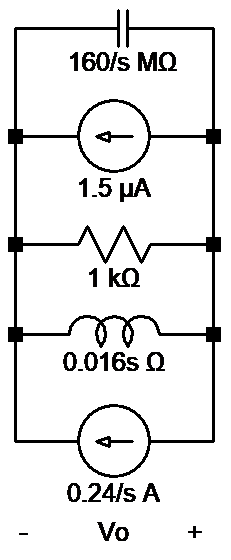
\includegraphics[width=0.2\linewidth]{A10-1.png}
\end{figure}

\item $Z_{eq}=\dfrac{16\cdot10^7}s\:\|\:1000\:\|\:0.016s,\quad I_{eq}=1.5\cdot10^{-6}+\dfrac{0.24}s$
\[V_o=-I_{eq}Z_{eq}=-\frac{1.5\cdot10^{-6}+\dfrac{0.24}s}{\dfrac1{\frac{16\cdot10^7}s}+\dfrac1{1000}+\dfrac1{0.016s}}=\boxed{-\frac{240s+38.4\cdot10^{6}}{s^2+160000s+10^{10}}\text{ V--s}}\]

\item $I_L=\dfrac{V_o}{0.016s}+\dfrac{0.24}s=\boxed{\dfrac{0.24s+23400}{s^2+160000s+10^{10}}\text{ A--s}}$

\item From (b), we have
\[V_o=-\frac{240s+38.4\cdot10^{6}}{s^2+160000s+10^{10}}=\frac{K_1}{s+80000-j60000}+\frac{K_1^*}{s+80000+j60000}\]
\[K_1=\left.\frac{-240s-38400000}{s+80000+j60000}\right|_{s=-80000+j60000}=200\phase{126.87^\circ}\]
\[\implies\boxed{v_o(t)=[400e^{-80000t}\cos(60000t+126.87^\circ)]u(t)\text{ A}}\]

\item From (b), we have
\[I_o=\dfrac{0.24s+23400}{s^2+160000s+10^{10}}=\frac{K_1}{s+80000-j60000}+\frac{K_1^*}{s+80000+j60000}\]
\[K_1=\left.\dfrac{0.24s+23400}{s+80000+j60000}\right|_{s=-80000+j60000}=0.125\phase{-16.26^\circ}\]
\[\implies\boxed{i_L(t)=[0.25e^{-80000t}\cos(60000t-16.26^\circ)]u(t)\text{ A}}\]

\end{enumerate}

\item The circuit in the $s$--domain:

\begin{figure}[H]
    \centering
    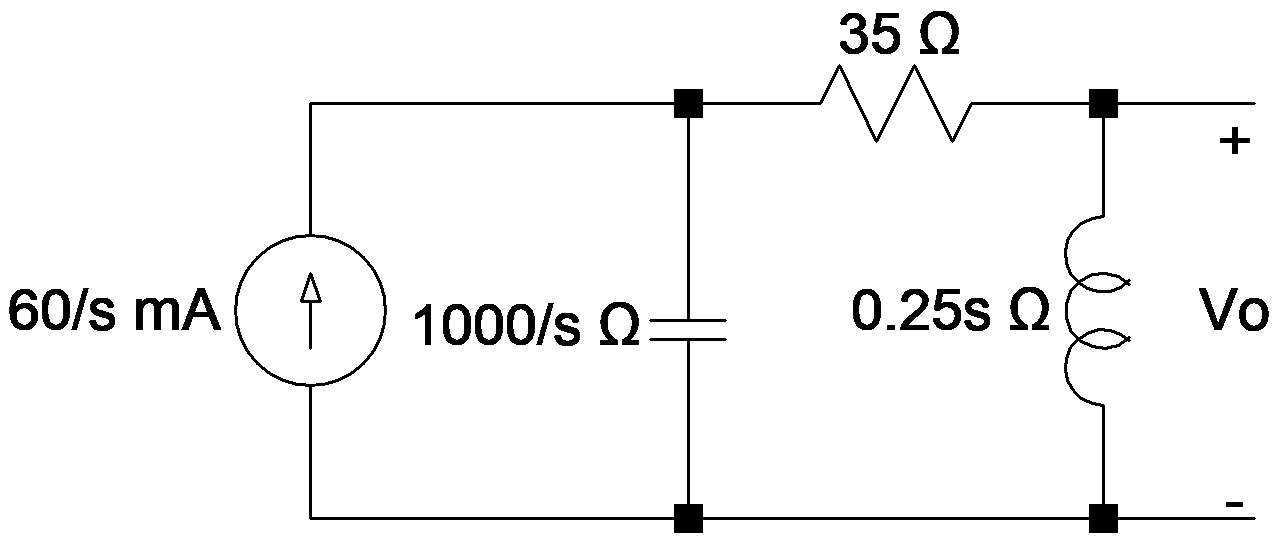
\includegraphics[width=0.55\linewidth]{A11-1.png}
\end{figure}

\begin{enumerate}[label=\textbf{\alph*)}]
\item $V_o=\dfrac{60}{s^2}\cdot\dfrac{0.25s}{\dfrac{1600}s+35+0.25s}=\dfrac{60}{s^2+140s+4000}$
\item $\displaystyle\lim_{t\to0}v_o(t)=\lim_{s\to\infty}sV_o(s)=\frac{s}{s^2+140s+4000}=0$

$\displaystyle\lim_{t\to\infty}v_o(t)=\lim_{s\to0}sV_o(s)=\frac{s}{s^2+140s+4000}=0.$
\[\boxed{v_o(0)=v_o(\infty)=0}\]

\item From (a), we have
\[V_o=\dfrac{60}{s^2+140s+4000}=\frac{K_1}{s+100}+\frac{K_2}{s+40} \quad[K_1=-1,\:K_2=1 \text{ directly}]\]
\[\boxed{v_o(t)=(e^{-40t}-e^{-100t})u(t)\text{ V}}\]

\end{enumerate}

\item The circuit in the $s$--domain:

\begin{figure}[H]
    \centering
    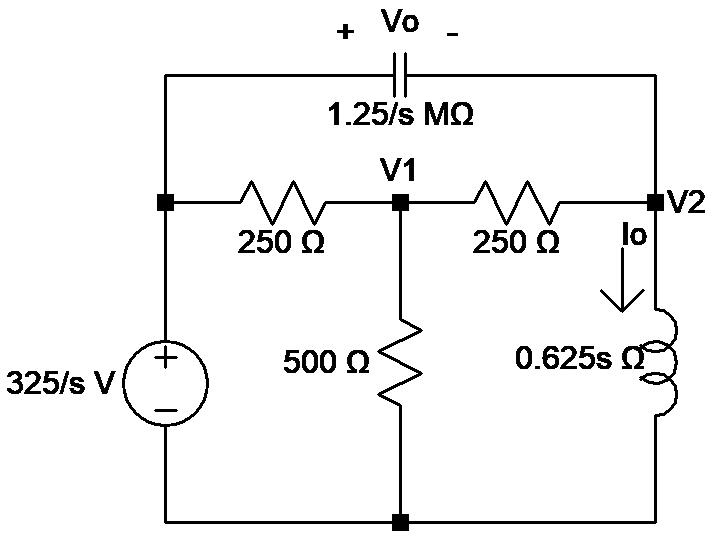
\includegraphics[width=0.45\linewidth]{A12-1.png}
\end{figure}

\begin{enumerate}[label=\textbf{\alph*)}]

\item From KCL equations,
\[\frac{V_1-\frac{325}s}{250}+\frac{V_1}{500}+\frac{V_1-V_2}{250}=0,\:\frac{V_2}{0.625s}+\frac{V_2-V_1}{250}+\frac{V_2-\frac{325}s}{1250000s}=0\implies 5V_1-2V_2=\frac{650}s\]
\[-5000sV_1+(s^2+5000s+2000000)V_2=325s\implies V_2=\frac{325}{s+1000}\]
\[\boxed{\begin{array}{rl}V_o&=\dfrac{325}s-\dfrac{325}{s+1000}\text{ V--s}\\[1em]I_o&=\dfrac{0.52}s-\dfrac{0.52}{s+1000}\text{ A--s}\end{array}}\]

\item Using the results in $(a)$,
\[\boxed{\begin{array}{rl}v_o(t)&=(325-325e^{-1000t})u(t)\text{ V}\\i_o(t)&=(520-520e^{-1000t})u(t)\text{ mA}\end{array}}\]

\item The poles of functions of $s$ lie on the $y$--axis and on the left of the axis, leading to constant and decaying exponential functions of $t$, which is feasible.

\end{enumerate}

\item The circuit in the $s$--domain:

\begin{figure}[H]
    \centering
    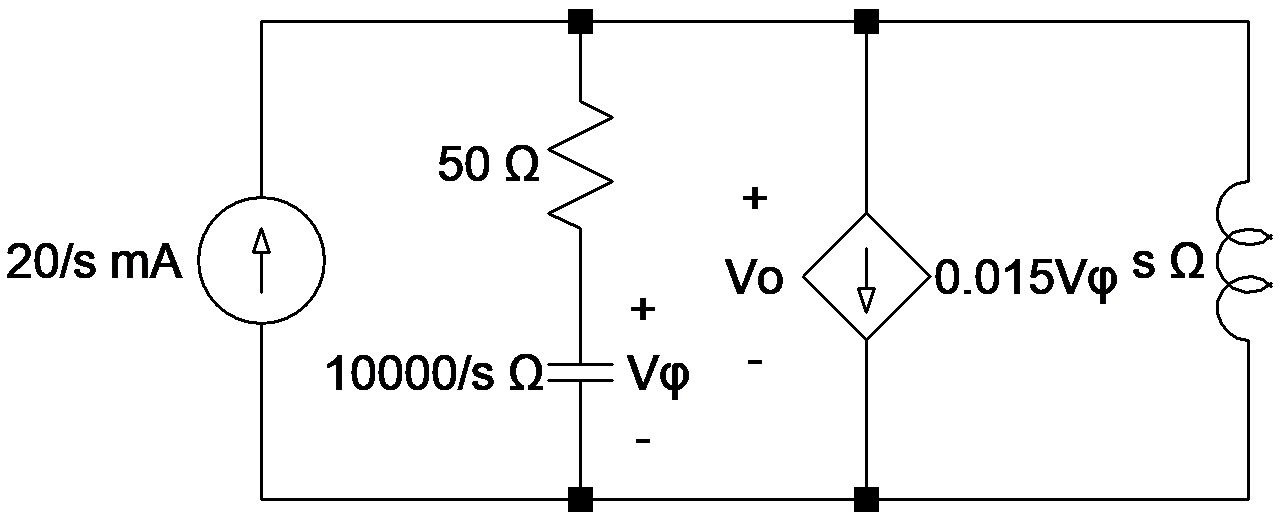
\includegraphics[width=0.55\linewidth]{A13-1.png}
\end{figure}

From KCL,
\[\frac{0.02}{s}+\frac{V_o}{50+10^4/s}+0.015V_\phi+\frac{V_o}s=0.\]

We have $V_\phi=\dfrac{\dfrac{10^4}s}{50+\dfrac{10^4}s}V_o=\dfrac{10^4\cdot V_o}{50s+10^4}$

Replacing $V_\phi$ in the KCL equation and solving for $V_o$, we get
\[V_o=\frac{s+200}{s^2+200s+10^4}=\frac{K_1}{(s+100)^2}+\frac{K_2}{s+100}\]
\[K_1=\left.(s+200)\right|_{s=-100}=100, \quad K_2=1\]
\[\implies\boxed{v_o(t)=(100te^{-100t}+e^{-100t})u(t)\text{ V}}\]

\item The $s$--domain equivalent circuit:

\begin{figure}[H]
    \centering
    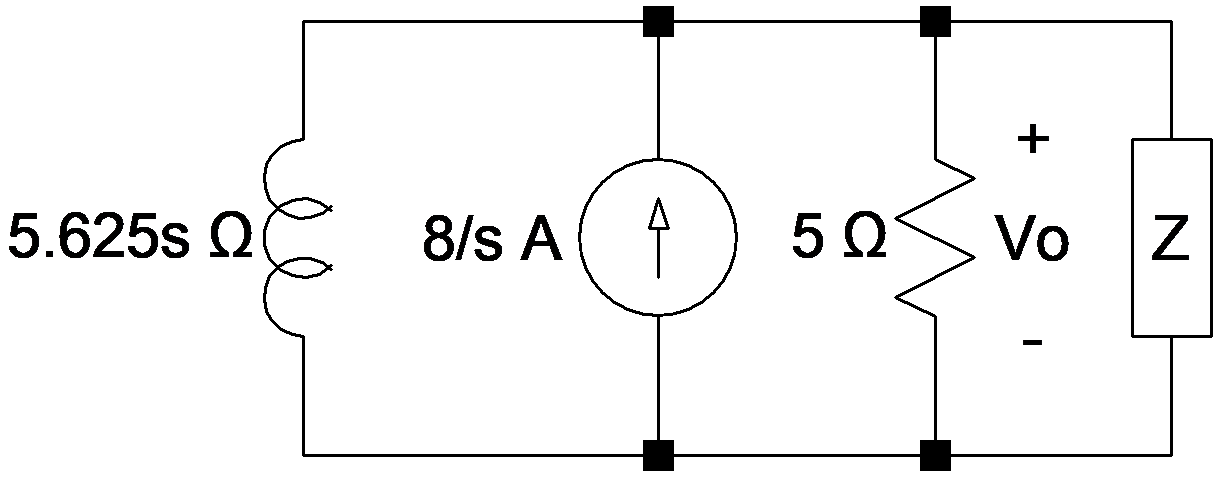
\includegraphics[width=0.5\linewidth]{A14-1.png}
\end{figure}

\begin{enumerate}[label=\textbf{\alph*)}]
\item Apply a test voltage to find the impedance to the right.

\begin{figure}[H]
    \centering
    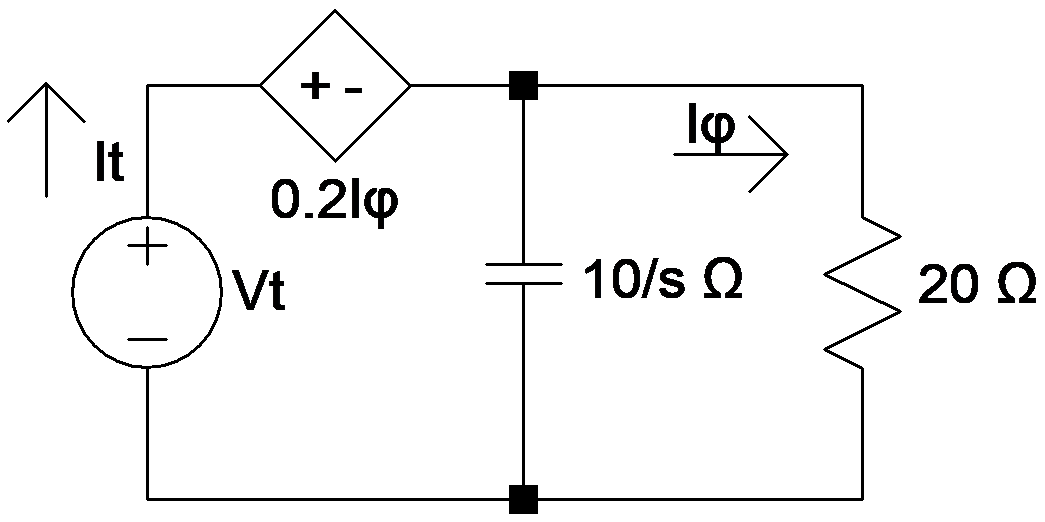
\includegraphics[width=0.55\linewidth]{A14-2.png}
\end{figure}

\[V_t=25I_\phi+\frac{20\cdot\dfrac{10}s}{20+\dfrac{10}s}I_t, \quad I_\phi=\frac{1+\dfrac{10}s}{20+\dfrac{10}s}\implies Z=\frac{V_t}{I_t}=\frac{250+200}{20s+10}=\frac{45}{2s+1}\]
\[\frac{V_o}s+\frac{V_o(2s+1)}{45}+\frac{V_o}{5.625s}=\frac8s\implies V_o=\frac{180}{s^2+5s+4}\text{ V--s}\]
\[V_1=\left.\frac{180}{s+1}\right|_{s=-4}=-60,\quad V_2=\left.\frac{180}{s+4}\right|_{s=-1}=60\implies\boxed{V_o=\frac{60}{s+1}-\frac{60}{s+4}\text{ V--s}}\]

\item $\boxed{v_o(t)=(60e^{-t}-60e^{-4t})u(t)\text{ V}}$

\end{enumerate}

\item Initially, we have
\[v_2(0^-)=450\cdot\frac{24\:\mu\:\|\: 16\:\mu}{24\:\mu\:\|\: 16\:\mu + 10\:\mu}=90\text{ V}\]

\begin{enumerate}[label=\textbf{\alph*)}]
\item The circuit:

\begin{figure}[H]
    \centering
    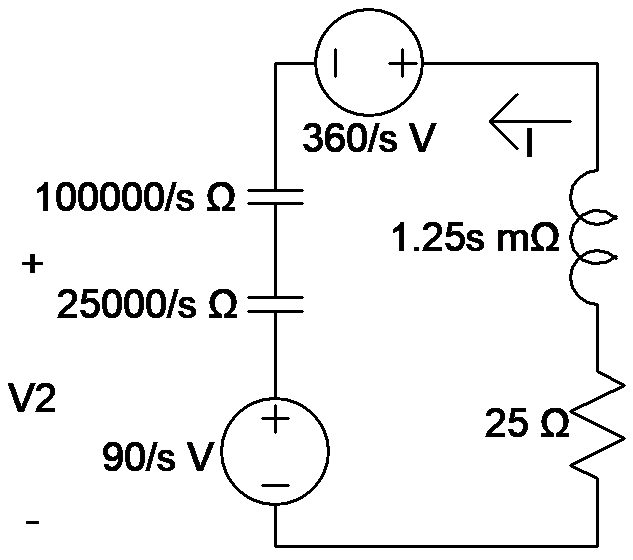
\includegraphics[width=0.4\linewidth]{A15-1.png}
\end{figure}

\item Let $I$ be the current in the counterclockwise direction.

$25I +1.25\cdot10^{-3}sI+\dfrac{450}s=0\implies I=\dfrac{-450s}{25+1.25\cdot10^{-3}s+\dfrac{125000}s}$

$\boxed{V_1=-25I=\dfrac{9000000}{(s+10000)^2}\text{ V--s}}$
\[K_1=90s+1800000|_{s=-10000}=900000,\quad K_2=90\]
\[\implies\boxed{v_1(t)=(9000000te^{-10000t})u(t)\text{ V}}\]

\item $v_2=I\cdot(25000/s)+90/s=\dfrac{90s+1800000}{s^2+20000s+10^8}=\dfrac{K_1}{(s+10000)^2}+\dfrac{K_2}{s+10000}$
\[K_1=90s+18\cdot10^5|_{s=-10000}=9\cdot10^5,\quad K_2=90\]
\[\boxed{V_2=\frac{900000}{(s+10000)^2}+\frac{90}{s+10000}\text{ V--s}}\]
\[\implies \boxed{v_2(t)=[900000te^{-10000t}+90e^{-10000t}]u(t)\text{ V}}\]

\end{enumerate}

\item \begin{enumerate}[label=\textbf{\alph*)}]
\item The circuit:

\begin{figure}[H]
    \centering
    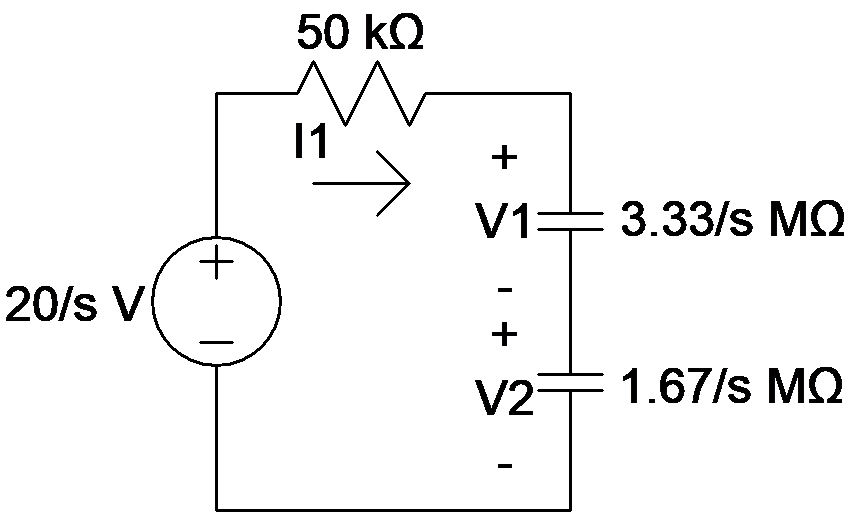
\includegraphics[width=0.5\linewidth]{A16-1.png}
\end{figure}

\item From KVL,
\[-\frac{20}s+50000I_1+\frac{5\cdot10^6I_1}s=0\implies \boxed{I_1=\frac{20}{5000000+50000s}=\frac{0.4\cdot10^{-3}}{s+100}\text{ A--s}}\]
\[\boxed{V_1=\frac{10}3\cdot\frac{10^6}s\cdot I=\frac{4000/3}{s(s+100)}\text{ V--s},\quad V_2=\frac{10^7}{6s}\cdot I=\frac{2000/3}{s(s+100)}\text{ V--s}}\]

\item $\boxed{I=(0.4\cdot10^{-3}e^{-100t})u(t)\text{ A}}$
\[V_1=\frac{K_1}s+\frac{K_2}{s+100}\implies K_1=\left.\frac{4000/3}{s+100}\right|_{s=0}=\frac{40}3,\:K_2=\left.\frac{4000/3}{s}\right|_{s=-100}=-\frac{40}3\]
\[\boxed{V_1=\frac{40}3(1-e^{-100t})u(t)\text{ V}, \quad V_2=\frac{V_1}2=\frac{20}3(1-e^{-100t})u(t)\text{ V}}\]

\item The poles of functions of $s$ lie on the $y$--axis and on the left of the axis, leading to constant and decaying exponential functions of $t$, which is physically meaningful.

\end{enumerate}

\item \begin{enumerate}[label=\textbf{\alph*)}]

\item The Laplace transform of $V_m\sin(\omega t+\phi)$:
\[\mathscr{L}\{V_m\sin(\omega t+\phi)\}=V_m\mathscr{L}\{\sin\omega t\cos\phi+\cos\omega t\sin\phi\}=\frac{\omega\cos\phi+s\sin\phi}{s^2+\omega^2}\]

%s-domain figure

\[I(s)=\frac{V_m\dfrac{\omega\cos\phi+s\sin\phi}{s^2+\omega^2}}{sL+R}=\frac{\frac{V_m}L(\omega\cos\phi+s\sin\phi)}{(s+\frac RL)(s^2+\omega^2)}=\frac{K_1}{s+\frac RL}+\frac{K_2}{s-j\omega}+\frac{K_2^*}{s+j\omega}\]
\[K_1=\left.\frac{\frac{V_m}L(\omega\cos\phi+s\sin\phi)}{s^2+\omega^2}\right|_{s=-\frac RL}=\frac{V_m(L\omega\cos\phi-R\sin\phi)}{R^2+\omega^2L^2}\]
\[ K_2=\left.\frac{\frac{V_m}L(\omega\cos\phi+s\sin\phi)}{\left(s+\frac RL\right)(s+j\omega)}\right|_{s=jw}=\frac{\frac{V_m}L(\omega\cos\phi+j\omega \sin\phi)}{\left(j\omega+\frac RL\right)2j\omega}=\frac{V_m(\cos\phi+j\sin\phi)}{(j\omega L+R)2j}\]
\[K_2=\dfrac{V_me^{j\phi}}{2\phase{90^\circ}\sqrt{\omega^2L^2+R^2}\phase{\tan^{-1}({\omega L/R})}}=\dfrac{V_m}{2\sqrt{\omega^2L^2+R^2}}\phase{\phi-90^\circ-\theta(\omega)}\]

\[\implies \boxed{i(t)=\underbrace{\frac{V_m(L\omega\cos\phi-R\sin\phi)}{\omega^2L^2+R^2}e^{-\frac RLt}}_{\text{Transient State}}+\underbrace{\frac{V_m\sin[\omega t+\phi-\theta(\omega)]}{\sqrt{\omega^2L^2+R^2}}}_{\text{Steady State}}\text{ A}}\]

\item $\boxed{\frac{V_m(L\omega\cos\phi-R\sin\phi)}{\omega^2L^2+R^2}e^{-\frac RLt}\text{ A}}$

\item $\boxed{\frac{V_m\sin[\omega t+\phi-\theta(\omega)]}{\sqrt{\omega^2L^2+R^2}}\text{ A}}$

\item $\mathbf{V}_g=\mathbf{I}(j\omega L+R)\implies\mathbf{I}=\dfrac{V_m\phase{\phi-90^\circ}}{\sqrt{\omega^2L^2+R^2}\phase{\theta(\omega)}}$
\[\implies\boxed{\Re(\mathbf{I})=\frac{V_m}{\sqrt{\omega^2L^2+R^2}}\sin[\omega t+\phi-\theta(\omega)]\text{ A}}\]

\item $L\omega\cos\phi=R\sin\phi\implies\boxed{\phi=\tan^{-1}\left(\dfrac{\omega L}{R}\right)}$

\end{enumerate}

\item Calculate $V_{th}$.

\begin{figure}[H]
    \centering
    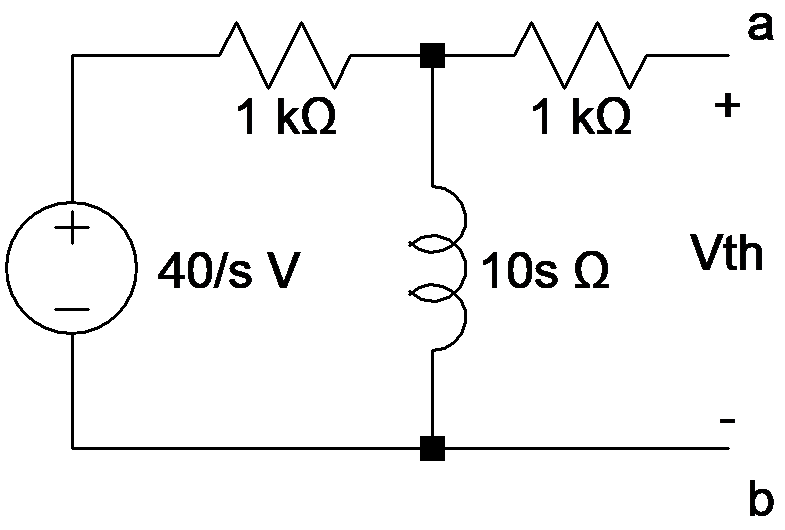
\includegraphics[width=0.4\linewidth]{A18-1.png}
\end{figure}

\[V_{th}=\dfrac{40}s\cdot\dfrac{10s}{10s+1000}=\dfrac{40}{s+100}\text{ V--s}\]

Calculate $Z_{th}$.

\begin{figure}[H]
    \centering
    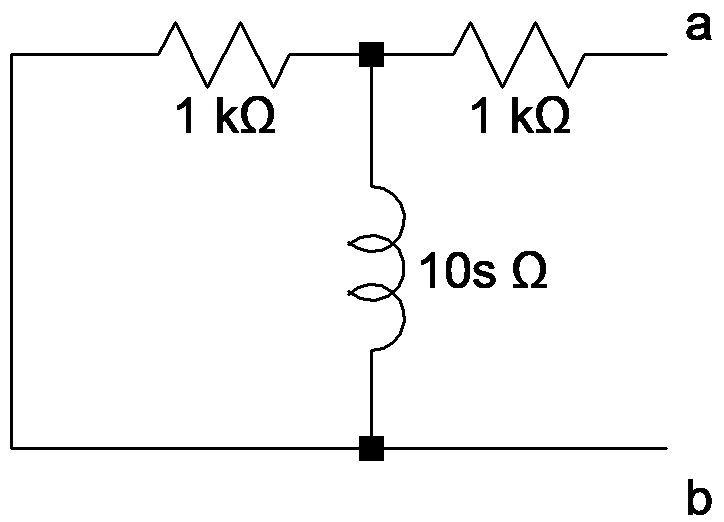
\includegraphics[width=0.35\linewidth]{A18-2.png}
\end{figure}

\[Z_{th}=1000+\frac1{\frac1{1000}+\frac1{10s}}=\frac{2000s+100000}{s+100}\]

%figure

\[I=\frac{\frac{40}{s+100}}{\frac{500000}s+\frac{2000s+1000}{s+100}}=\frac{40s}{2000s^2+600000s+5000000}=\frac{0.02s}{s^2+30s+25000}\]
\[I=\frac{K_1}{s+150-j50}+\frac{K_1^*}{s+150+j50}\]
\[\implies K_1=\left.\frac{0.02s}{s+150+j50}\right|_{s=-150+j50}=31.62\cdot10^{-3}\phase{71.57^\circ}\]
\[\implies\boxed{i(t)=[63.24e^{-150t}\cos(50t+71.57^\circ)]u(t) \text{ mA}}\]

\item \begin{enumerate}[label=\textbf{\alph*)}] 

\item Let $I_1$ and $I_2$ circulate clockwise in the left and right meshes, respectively.
\[(100+0.1875s)I_1+0.125sI_2-\frac{150}s=0\quad \text{and}\quad 0.125sI_1+(200+0.25s)I_1=0\]

Solve the latter equation for $I_1$ and substitute into the former equation, then
\[\implies\boxed{I_1(s)=\frac{1200(s+800)}{s(s^2+2000s+640000)}\text{ A--s}}\]

\item $\displaystyle \boxed{i_1(0)=\lim_{s\to\infty}sI_1=0,\quad \lim_{t\to\infty}i_1(t)=\lim_{s\to0}sI_1=1.5\text{ A}}$

\item $I_1=\dfrac{K_1}{s}+\dfrac{K_2}{s+400}+\dfrac{K_3}{s+1600}$
\[K_1=\left.\frac{1200(s+800)}{(s^2+1000s+640000)}\right|_{s=0}=1.5,\quad K_2=\left.\frac{1200(s+800)}{s(s+1600)}\right|_{s=-400}=-1,\]
\[K_3=\left.\frac{1200(s+800)}{s(s+400)}\right|_{s=-1600}=-0.5\implies \boxed{i_1(t)=(1.5-e^{-400t}-0.5e^{-1600t})u(t)\text{ A}}\]

\end{enumerate}

\
\item \begin{enumerate}[label=\textbf{\alph*)}] 

\item The $s$--domain equivalent circuit:

\begin{figure}[H]
    \centering
    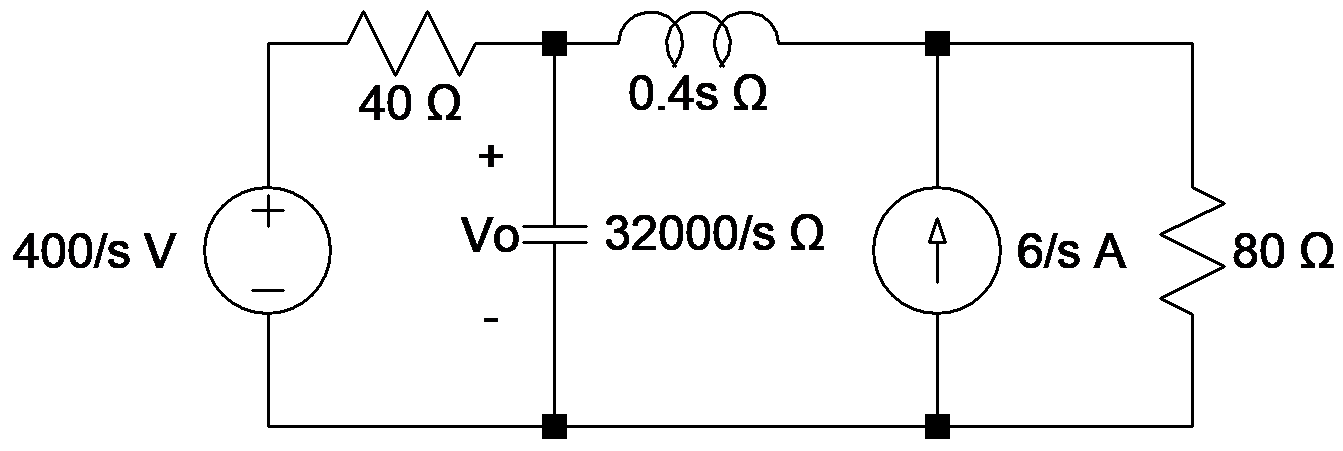
\includegraphics[width=0.65\linewidth]{A20-1.png}
\end{figure}

Zero the current source to find the individual response of the voltage source.

\begin{figure}[H]
    \centering
    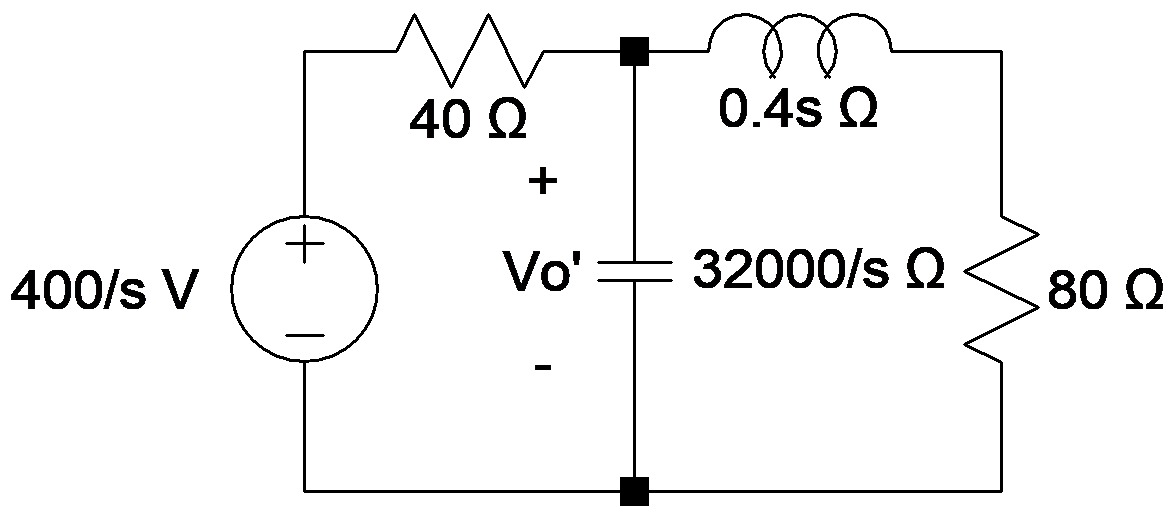
\includegraphics[width=0.55\linewidth]{A20-2.png}
\end{figure}

\[V_o'=\frac{400}s\cdot\frac{{\dfrac{(0.4s+80)\cdot\frac{32000}s}{0.4s+80+\frac{32000}s}}}{40+\dfrac{(0.4s+80)\cdot\frac{32000}s}{0.4s+80+\frac{32000}s}}=\frac{320000(s+200)}{s(s^2+1000s+240000)}\]

Zero the voltage source.

\begin{figure}[H]
    \centering
    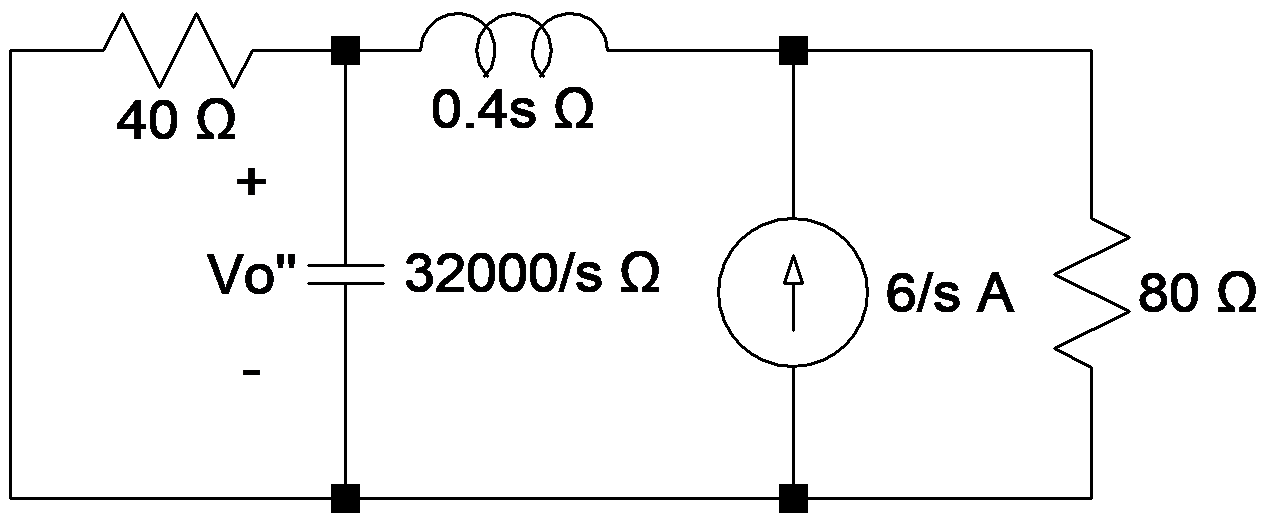
\includegraphics[width=0.55\linewidth]{A20-3.png}
\end{figure}

\[I''=\frac{80}{\left(\frac{32000}{s}\:\|\:40\right)+0.4s+80}\cdot\frac6s=\frac{480(s+800)}{s(0.4s^2+400s+96000)}\]
\[V_o''=\frac{1200(s+800)}{s(s^2+1000s+240000)}\cdot\left(\frac{32000}{s}\:\|\:40\right)=\frac{38400000}{s(s^2+1000s+240000)}\]

\[\implies \boxed{V_o=V_o'+V_o''=\frac{320000(s+320)}{s(s^2+1000s+240000)}\text{ V--s}}\]

\item $V_o=\dfrac{K_1}{s}+\dfrac{K_2}{s+400}+\dfrac{K_3}{s+600}$.
\[K_1=\left.\frac{320000(s+320)}{s^2+1000s+240000}\right|_{s=0}=\frac{1280}3,\quad K_2=\left.\frac{320000(s+320)}{s(s+600)}\right|_{s=-400}=320\]
\[K_3=\left.\frac{320000(s+320)}{s(s+400)}\right|_{s=600}=-\frac{2240}3\]
\[\implies\boxed{V_o(t)=\left(\frac{1280}3+320e^{-400t}-\frac{2240}3e^{-600t}\right)u(t)\text{ V}}\]

\end{enumerate}

\end{enumerate}

\end{document}